\subsection{Android Interface}
	This section displays the envisioned design of the Android Application layout.

	\subsubsection{New Site Visit}
		\begin{center}
			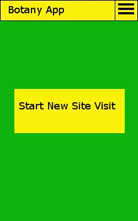
\includegraphics[scale=1]{uiDesign/botanyAppNewSiteVisit1.png}
			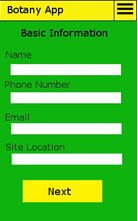
\includegraphics[scale=1]{uiDesign/botanyAppNewSiteVisit2.png}
		\end{center}
	
		The first thing that will be presented to the user on entry to the app will be the option to create a new visit by pushing the button provided. This will then load the Basic Information page.\\

		The user will then be prompted to input their basic information such as their name, phone number, email and site location for reference. These are to be validated by the server upon the push of the Next button. Add a species page will then be displayed to the user.\\
	
		Further fields may be required to be added at a later date due to additional requirements given by the client or by a change during further development in the design.\\
	
		There is no requirement in the spec to remember the user’s details on the app so currently the user will have to fill in their details each time they make a recording.\\
		
	\subsubsection{Adding a new species}
		\begin{center}
			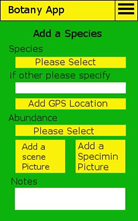
\includegraphics[scale=1]{uiDesign/botanyAppAddSpecies1.png}
			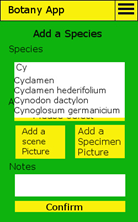
\includegraphics[scale=1]{uiDesign/botanyAppAddSpecies2.png}
		\end{center}
		The first input asked of the user is to select a species to record using an integrated search function. This will not only help the user find the species they are looking for, but also allow the user to add a new species to the database if required.\\
		
		An option to provide a GPS signal is given which will link up with the GPS in the android device to provide a location. Options are given to provide pictures of the site and specimen either from the camera or the gallery on the device. A field for adding notes will be provided that may be useful to the record.\\
	
	\subsubsection{Editing and saving a site visit}
		\begin{center}
			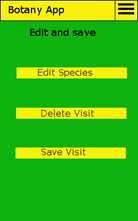
\includegraphics[scale=1]{uiDesign/botanyAppEditSaveSiteVisit.png}
		\end{center}
		The edit and save page provides the options to the user to view and edit the recordings made. The Edit Species link allows the user to access a list of the species pages they have added to the visit. This takes the user back to the Add a Species page to edit or delete an entry.\\
		
		Users are given the option to delete the visit which will be met with a prompt to confirm or cancel the delete.\\

		The final link is to save all recordings, giving permission to upload the data to the database at an appropriate time.\\
		
	\subsection{Web Interface}
		This section displays the envisioned design of the Website Layout

		\subsubsection{Web Homepage}
			\begin{center}
				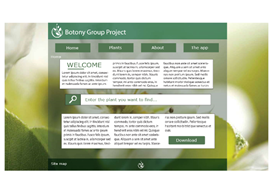
\includegraphics[scale=1]{uiDesign/botanyWebHome.png}
			\end{center}
		The Homepage has a central search bar to search the database for visit records and species information. The navigation bar at the top remains consistent over all pages with breadcrumbs just below to ensure ease of navigation. There is a link to the site map in the footer which also remains consistent. There will be a heading welcoming the user, alongside information regarding the nature and purpose of the website. 

		\subsubsection{Plant Database Page}
			\begin{center}
				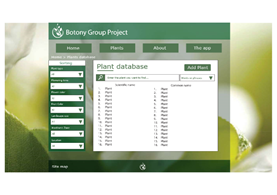
\includegraphics[scale=1]{uiDesign/botanyWebPlantDatabase.png}
			\end{center}
		The plant database provides access to the entire database using the search bar to search plants by name. The search results will be displayed as a list. At the side there is a sorting bar which contains various drop down menus of search filters to refine the search if required. The user can then click a record which will be linked to the plants details (4.7). The Add Plant button will link the user to the Add record page.

		\subsubsection{Add Record Page}
			\begin{center}
				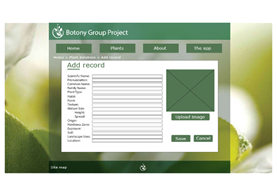
\includegraphics[scale=1]{uiDesign/botanyWebAddRecord.png}
			\end{center}
		This page allows the user to add a new record to the database. The user will be asked to provide information such as scientific name, pronunciation, common name, origin and location alongside an image that can be uploaded to the database upon clicking the save button. 
		
		\subsubsection{Plant Details Overlay}
			\begin{center}
				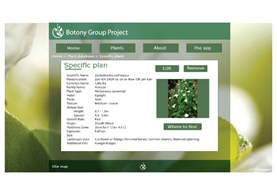
\includegraphics[scale=1]{uiDesign/botanyWebPlantDetailsOverlay.png}
			\end{center}
			The specific plant page allows the user to access data about individual plants. Above the picture there are links to edit and remove the records giving the user the ability to update the data about the plant. A where to find button links to a map of the location based from GPS coordinates.

			\subsubsection{Plant Location Overlay}
			\begin{center}
				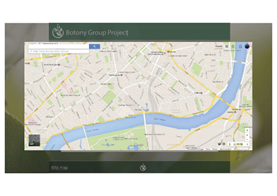
\includegraphics[scale=1]{uiDesign/botanyWebPlantMap.png}
			\end{center}
			Upon clicking the Where to Find button, a map will open displaying the location of the selected plant using the location from the database. Note: Use of Google Maps.

		\subsubsection{Remove Plant Record}
			\begin{center}
				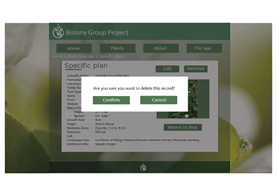
\includegraphics[scale=1]{uiDesign/botanyWebPlantRemoval.png}
			\end{center}
			If the user chooses to remove a record they can do so by pressing the Remove button where they will be prompted to verify their choice before the entry is deleted.